% !TeX root = Stageportfolio.tex



\begin{landscape}
	\subsubsection{Les 17-18}
	\begin{tabularx}{1.56\textwidth}{|p{0.35\textwidth}|X|}\hline
		\textbf{Administratieve gegevens}\newline\newline
		Kevin Truyaert\newline\newline
		technisch secundair onderwijs\newline
		3e graad, 1ste jaar, Techniek-Wetenschappen\newline
		VVKSO: \href{http://ond.vvkso-ict.com/leerplannen/doc/Toegepaste\%20fysica-2014-041.pdf}{http://ond.vvkso-ict.com/leerplannen /doc/Toegepaste\%20fysica-2014-041.pdf} \newline
		\underline{Lesonderwerp}:\newline Oefeningen op de algemene inductiewet \& Toepassingen op inductie & \textbf{Doelstellingen}
		\begin{itemize}[itemsep=0.08\baselineskip]
			\item B27: Fluxverandering als oorzaak van inductiespanning toelichten.
			\item B28: Met behulp van de wet van Lenz de zin van de inductiespanning vinden.
			\item B29: De algemene inductiewet hanteren.
			\item B30: Het werkingsprincipe van een generator weergeven.
		\end{itemize}
		\underline{Lesdoelen}\newline
		\vspace{-0.75cm}
		\begin{enumerate}[itemsep=0.08\baselineskip]
			\item De leerlingen kunnen de wet van Faraday-Lenz op een rechte, bewegende geleider toepassen.
			\item De leerlingen kennen de relatie tussen inductiespanning, magnetisch veld, lengte van de geleider, snelheid van de geleider en aantal windingen.
			\item De leerlingen kunnen de algemene inductiewet tijdens oefeningen hanteren.
			\item De leerlingen kunnen de werking van een wisselspanningsgenerator weergeven.
		\end{enumerate} \\\hline
	\end{tabularx}\vfill \textcolor{white}{.} 


	\begin{tabularx}{1.56\textwidth}{|p{0.55\textwidth}|X|}
		\hline
		\multirow{2}{0.55\textwidth}{\textbf{Beginsituatie}\newline  
		Er zijn acht leerlingen binnen 5TW. Er heerst een algemene klassfeer. De leerlingen hebben al theorie gekregen rond en basisoefeningen gemaakt op magnetische inductie.  \newline\newline NOG AANVULLEN MET LERAARKENMERKEN.} & \textbf{Acties}\newline\newline  
		- Ik wil oefeningen op zo'n wijze brengen dat ze steeds dezelfde structuur hebben. Die structuur bouw ik eerst samen met de leerlingen op, om ze daarna zelfstandig aan de slag te laten gaan met oefeningen die steeds wat complexer worden. \PinkHighlight{Tijdens het zelfstandig maken van de oefeningen probeer ik toch zeker}{13cm} \PinkHighlight{de zwakkere leerlingen in de gaten te houden en hen individueler te coachen bij het}{15cm} \PinkHighlight{maken van oefeningen.}{4.5cm}
		\newline\newline\newline\newline\newline\newline\newline\newline
		
		\\ \cline{2-2}
		  & \textbf{Bronnen}\begin{itemize}
		  	\item Schramme, S. (2018) De stroombalans, labo magnetisme 4
		  	\item Frederiksen (2014), Current Balance 4565.00
		  	\item Giancoli, D. C. (2008). Physics for scientists and engineers. Pearson Education International.
		  \end{itemize}\\ \hline
	\end{tabularx}


\newpage
	
	\begin{tabularx}{1.56\textwidth}{|p{1.5cm}|p{8cm}|X|p{4cm}|}
		\hline
		\textbf{Nr. lesdoel } & \textbf{Inhoud (timing)}  & \textbf{Organisatie } & \textbf{Media } \\ \hline
		1\newline\newline2\newline\newline3	&\underline{Oefeningen: de algemene} \underline{inductiewet (40 minuten)}\newline
			Tijdens deze lesfase focussen de leerlingen zich op het maken van oefeningen in verband met de algemene inductiewet. Deze combineert de wet van Faraday en de wet van Lenz, dus leerlingen moeten beide begrijpen om de oefeningen tot een goed einde te brengen. Tijdens deze oefeningensessie wil ik gebruik maken van correctiesleutels om de leerlingen hun oefeningen zelfstandig te laten corrigeren.
		&  \underline{Zelfstandig oefeningen maken} \underline{Bespreking via correctiesleutel}\newline 
			De leerlingen maken zelfstandig oefeningen 6 t.e.m. 11. Na het maken van iedere oefening kunnen ze een correctiesleutel ophalen waarin alle stappen beschreven staan. Zo kunnen de sterkere leerlingen zelfstandig meerdere (en complexere) oefeningen maken, terwijl ik mij concentreer op de zwakkere leerlingen. Wanneer ik zie dat er bij een bepaalde oefening klassikaal problemen zijn, kan ik bepaalde stappen op het bord brengen.
		&   Cursus hoofdstuk 5 p15-16\newline\newline Krijtbord
		\\ \hline
	\end{tabularx}\vspace{5mm}



\begin{tabularx}{1.56\textwidth}{|p{1.5cm}|p{8cm}|X|p{4cm}|}
	\hline
	\textbf{Nr. lesdoel } & \textbf{Inhoud (timing)}  & \textbf{Organisatie } & \textbf{Media } \\ \hline
    4 & \underline{Werking wisselspanningsgenerator:} \underline{inleiding (5 minuten)}\newline
    	Opzet van de wisselspanningsgenerator verduidelijken en kennismaken met de werking ervan.
	&  \underline{Onderwijsleergesprek}\newline 
	Ik schets de opstelling van de wisselspanningsgenerator en vraag de leerlingen om alle componenten aan te duiden, te benoemen, \ldots 
	&  Cursus hoofdstuk 6 p6\newline\newline Slides
	\\ \hline
\end{tabularx}\vspace{5mm}


\begin{tabularx}{1.56\textwidth}{|p{1.5cm}|p{8cm}|X|p{4cm}|}
	\hline
	\textbf{Nr. lesdoel } & \textbf{Inhoud (timing)}  & \textbf{Organisatie } & \textbf{Media } \\ \hline
	4& \underline{Werking wisselspanningsgenerator:} \underline{eerste kwartdraai (5 minuten)}\newline
	De werking van de wisselspanningsgenerator wordt verduidelijkt. Dit zal in verschillende stappen gebeuren.
	&  \underline{Onderwijsleergesprek}\newline  De leerlingen kennen de werking van de algemene inductiewet. Via vraagstelling wil ik samen met hen de eerste kwartdraai van de wisselspanningsgenerator bespreken. Zo vullen we samen het eerste kader op pagina 7 in.
	&  Cursus hoofdstuk 6 p7\newline\newline Krijtbord
	\\ \hline
\end{tabularx}\vspace{5mm}


\begin{tabularx}{1.56\textwidth}{|p{1.5cm}|p{8cm}|X|p{4cm}|}
\hline
\textbf{Nr. lesdoel } & \textbf{Inhoud (timing)}  & \textbf{Organisatie } & \textbf{Media } \\ \hline
4& \underline{Werking wisselspanningsgenerator:} \underline{volgende kwartdraaien (5 minuten)}\newline
De leerlingen bepalen zelf het verloop van één van de kwartdraaien. 
&  \underline{Zelfstandig werk}\newline  Ik zet de leerlingen met hun buur aan de slag, per twee. Zo ontstaan er vier groepjes. Ik geef de leerlingen een getal (2, 3 of 4). Het is de bedoeling dat de leerlingen zelfstandig die kwartdraai proberen te beschrijven. Indien ze klaar zijn met hun kwartdraai, kunnen ze nog de andere zelfstandig proberen te maken. Ik geef al de aanzet bij alle drie de gevallen door de begin- en eindhoek van de beweging mee te geven.
&  Cursus hoofdstuk 6 p7-8
\\ \hline
\end{tabularx}\vspace{5mm}

\begin{tabularx}{1.56\textwidth}{|p{1.5cm}|p{8cm}|X|p{4cm}|}
	\hline
	\textbf{Nr. lesdoel } & \textbf{Inhoud (timing)}  & \textbf{Organisatie } & \textbf{Media } \\ \hline
	4& \underline{Werking wisselspanningsgenerator:} \underline{volgende kwartdraaien (5 minuten)}\newline
	De leerlingen bepalen zelf het verloop van één van de kwartdraaien. 
	&  \underline{Zelfstandig werk}\newline  Ik zet de leerlingen met hun buur aan de slag, per twee. Zo ontstaan er vier groepjes. Ik geef de leerlingen een getal (2, 3 of 4). Het is de bedoeling dat de leerlingen zelfstandig die kwartdraai proberen te beschrijven. Indien ze klaar zijn met hun kwartdraai, kunnen ze nog de andere zelfstandig proberen te maken. Ik geef al de aanzet bij alle drie de gevallen door de begin- en eindhoek van de beweging mee te geven.
	&  Cursus hoofdstuk 6 p7-8
	\\ \hline
\end{tabularx}\vspace{5mm}


\begin{tabularx}{1.56\textwidth}{|p{1.5cm}|p{8cm}|X|p{4cm}|}
	\hline
	\textbf{Nr. lesdoel } & \textbf{Inhoud (timing)}  & \textbf{Organisatie } & \textbf{Media } \\ \hline
	4& \underline{Werking wisselspanningsgenerator:} \underline{volledige werking (15 minuten)}\newline
	De leerlingen overlopen het verloop van de wisselspanningsgenerator met elkaar. 
	&  \underline{Zelfstandig werk + onderwijsleergesprek}\newline  Ik laat verschillende leerlingen aan het woord om hun casus te bespreken en die te delen met hun medeleerlingen. Zo zal iedereen het volledige verloop beet hebben. Ik zorg dat iedere leerling aan bod gekomen is. Ik eindig met de werking van de wisselspanningsgenerator nog eens met een video samen te vatten.
	&  Cursus hoofdstuk 6 p7-8 \newline\newline Projectie
	\\ \hline
\end{tabularx}\vspace{5mm}



\begin{tabularx}{1.56\textwidth}{|p{1.5cm}|p{8cm}|X|p{4cm}|}
	\hline
	\textbf{Nr. lesdoel } & \textbf{Inhoud (timing)}  & \textbf{Organisatie } & \textbf{Media } \\ \hline
	4& \underline{Werking wisselspanningsgenerator:} \underline{verloop flux en inductiespanning} \underline{(8 minuten)}\newline
	De leerlingen hebben net de volledige werking van de wisselspanningsgenerator doorlopen. Hieruit kunnen ze enkele punten uitzetten van de flux in functie van de tijd en de inductiespanning in functie van de tijd. 
	&  \underline{Zelfstandig werk + onderwijsleergesprek}\newline  
	Ik vraag de leerlingen om na te denken over het verloop van de flux en de inductiespanning bij de wisselspanningsgenerator. Ik vraag hen om enkele punten in potlood uit te zetten, te beginnen van een situatie waaarbij de spoel horizontaal en het magnetisch veld verticaal ligt. Ik toon de startsituatie en de draairichting via projectie. Daarna laat ik hen aan de slag gaan en teken ik zelf de assen van mijn grafiek op bord. Daarna vraag ik de leerlingen welke punten ze gevonden hebben bij de situatie en breng ik die aan het bord. Ik vraag `waarom' zowel bij foutieve als correcte antwoorden.
	&  Cursus hoofdstuk 6 p9 \newline\newline Projectie\newline\newline Bord
	\\ \hline
\end{tabularx}\vspace{5mm}



\begin{tabularx}{1.56\textwidth}{|p{1.5cm}|p{8cm}|X|p{4cm}|}
	\hline
	\textbf{Nr. lesdoel } & \textbf{Inhoud (timing)}  & \textbf{Organisatie } & \textbf{Media } \\ \hline
	4& \underline{Werking wisselspanningsgenerator:} \underline{besluit(7 minuten)}\newline
	De leerlingen hebben net de volledige werking van de wisselspanningsgenerator doorlopen. We bespreken nu het besluit hiervan. Hoe gebeurt de energieoverdracht?
	&  \underline{Onderwijsleergesprek}\newline  
	We overlopen nog een laatste maal samen wat er juist gebeurd bij een wisselspanningsgenerator. We bespreken vooral hoe de energie overzetting gebeurd. Ook leg ik hier nog eens de nadruk tussen wat het verschil tussen en motor en een generator is.	
	&  Cursus hoofdstuk 6 p9-10 \newline\newline Projectie\newline\newline Bord
	\\ \hline
\end{tabularx}\vspace{5mm}




\begin{tabularx}{1.56\textwidth}{|p{1.5cm}|p{8cm}|X|p{4cm}|}
	\hline
	\textbf{Nr. lesdoel } & \textbf{Inhoud (timing)}  & \textbf{Organisatie } & \textbf{Media } \\ \hline
	5& \underline{Werking transformator:} \underline{inleiding (10 minuten)}\newline
	 Ik leid in wat een transformator juist is. Dit is belangrijk, omdat we hier woensdag op verder zullen bouwen. Verder is er op donderdag ook nog een labo in verband met de transformator. Het is daarom belangrijk dat dit in de theorie nog besproken wordt.
	&  \underline{Doceren - onderwijsleergesprek}\newline 
	Dit laatste stukje zal ik eerder op een docerende manier behandelen. De introductie van een transformator is niet eenvoudig, er zijn een heleboel componenten die benoemd moeten worden met de correcte terminologie (primaire - secundaire). Hierbij wil ik vooral spreken over de bouw en het doel van de transfo. Ik kies er hier voor om geen slot met herhaling van de les in te bouwen gezien er net de conclusie van de wisselspanningsgenerator gebeurd is. 	
	&  Cursus hoofdstuk 6 p11 \newline\newline Projectie\newline\newline Bord
	\\ \hline
\end{tabularx}\vspace{5mm}




	
\end{landscape}


%\subsection*{Bijlage 5.1: slides introductie}

%
%\subsection*{Bijlage 1.2: bordschema theorie}
%\begin{center}
%	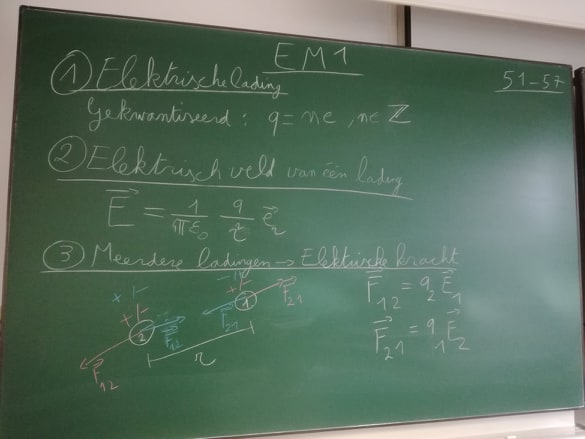
\includegraphics[width=0.9\textwidth]{Bord1a}
%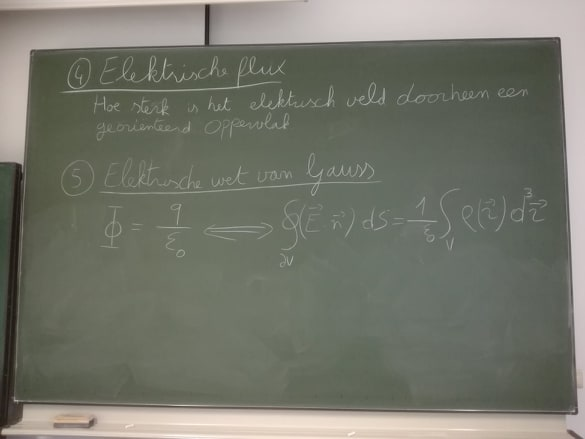
\includegraphics[width=0.9\textwidth]{Bord1b}
%\end{center}
%\newpage
%
%
%\includepdf[scale = 0.8,pages = 17,pagecommand=\subsection*{Bijlage 1.3: opgeloste oefeningen}]{Observaties_OpgelosteOef}
%\includepdf[scale = 0.8,pages =18-20,pagecommand=]{Observaties_OpgelosteOef}
%
%
%
%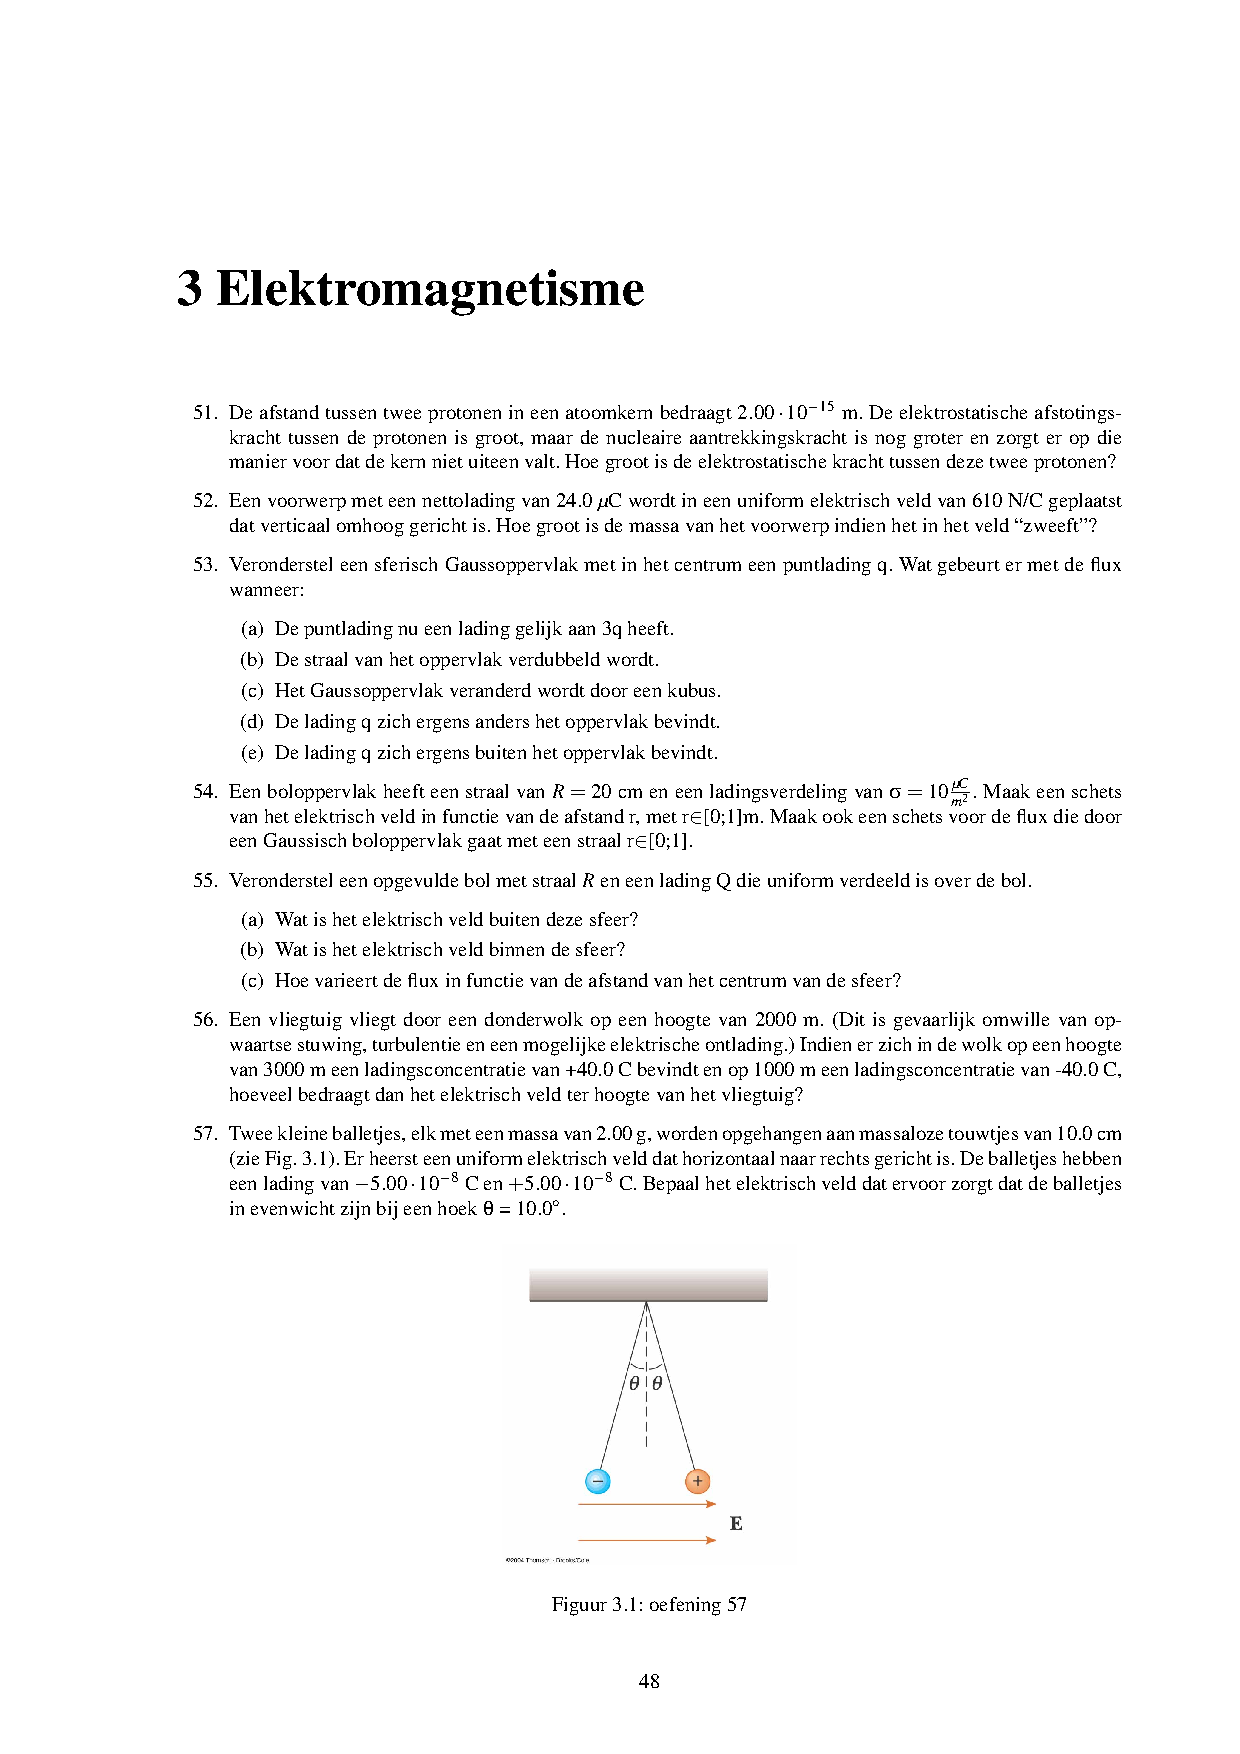
\includepdf[scale = 0.95,pages = 1,pagecommand=\subsection*{Bijlage 1.4: oefeningenbundel elektromagnetisme}]{OefeningenBundel}
%\includepdf[scale = 0.95,pages =2-,pagecommand=]{OefeningenBundel}